%\newpage
\section{Обработка результатов измерений}
\subsection{Результаты измерений}
Приведем графики полученных спектров (рис. \ref{full_03_279}--\ref{full_04_515}).
\begin{figure}[H]
	\begin{minipage}{0.45\linewidth}
		\centering
		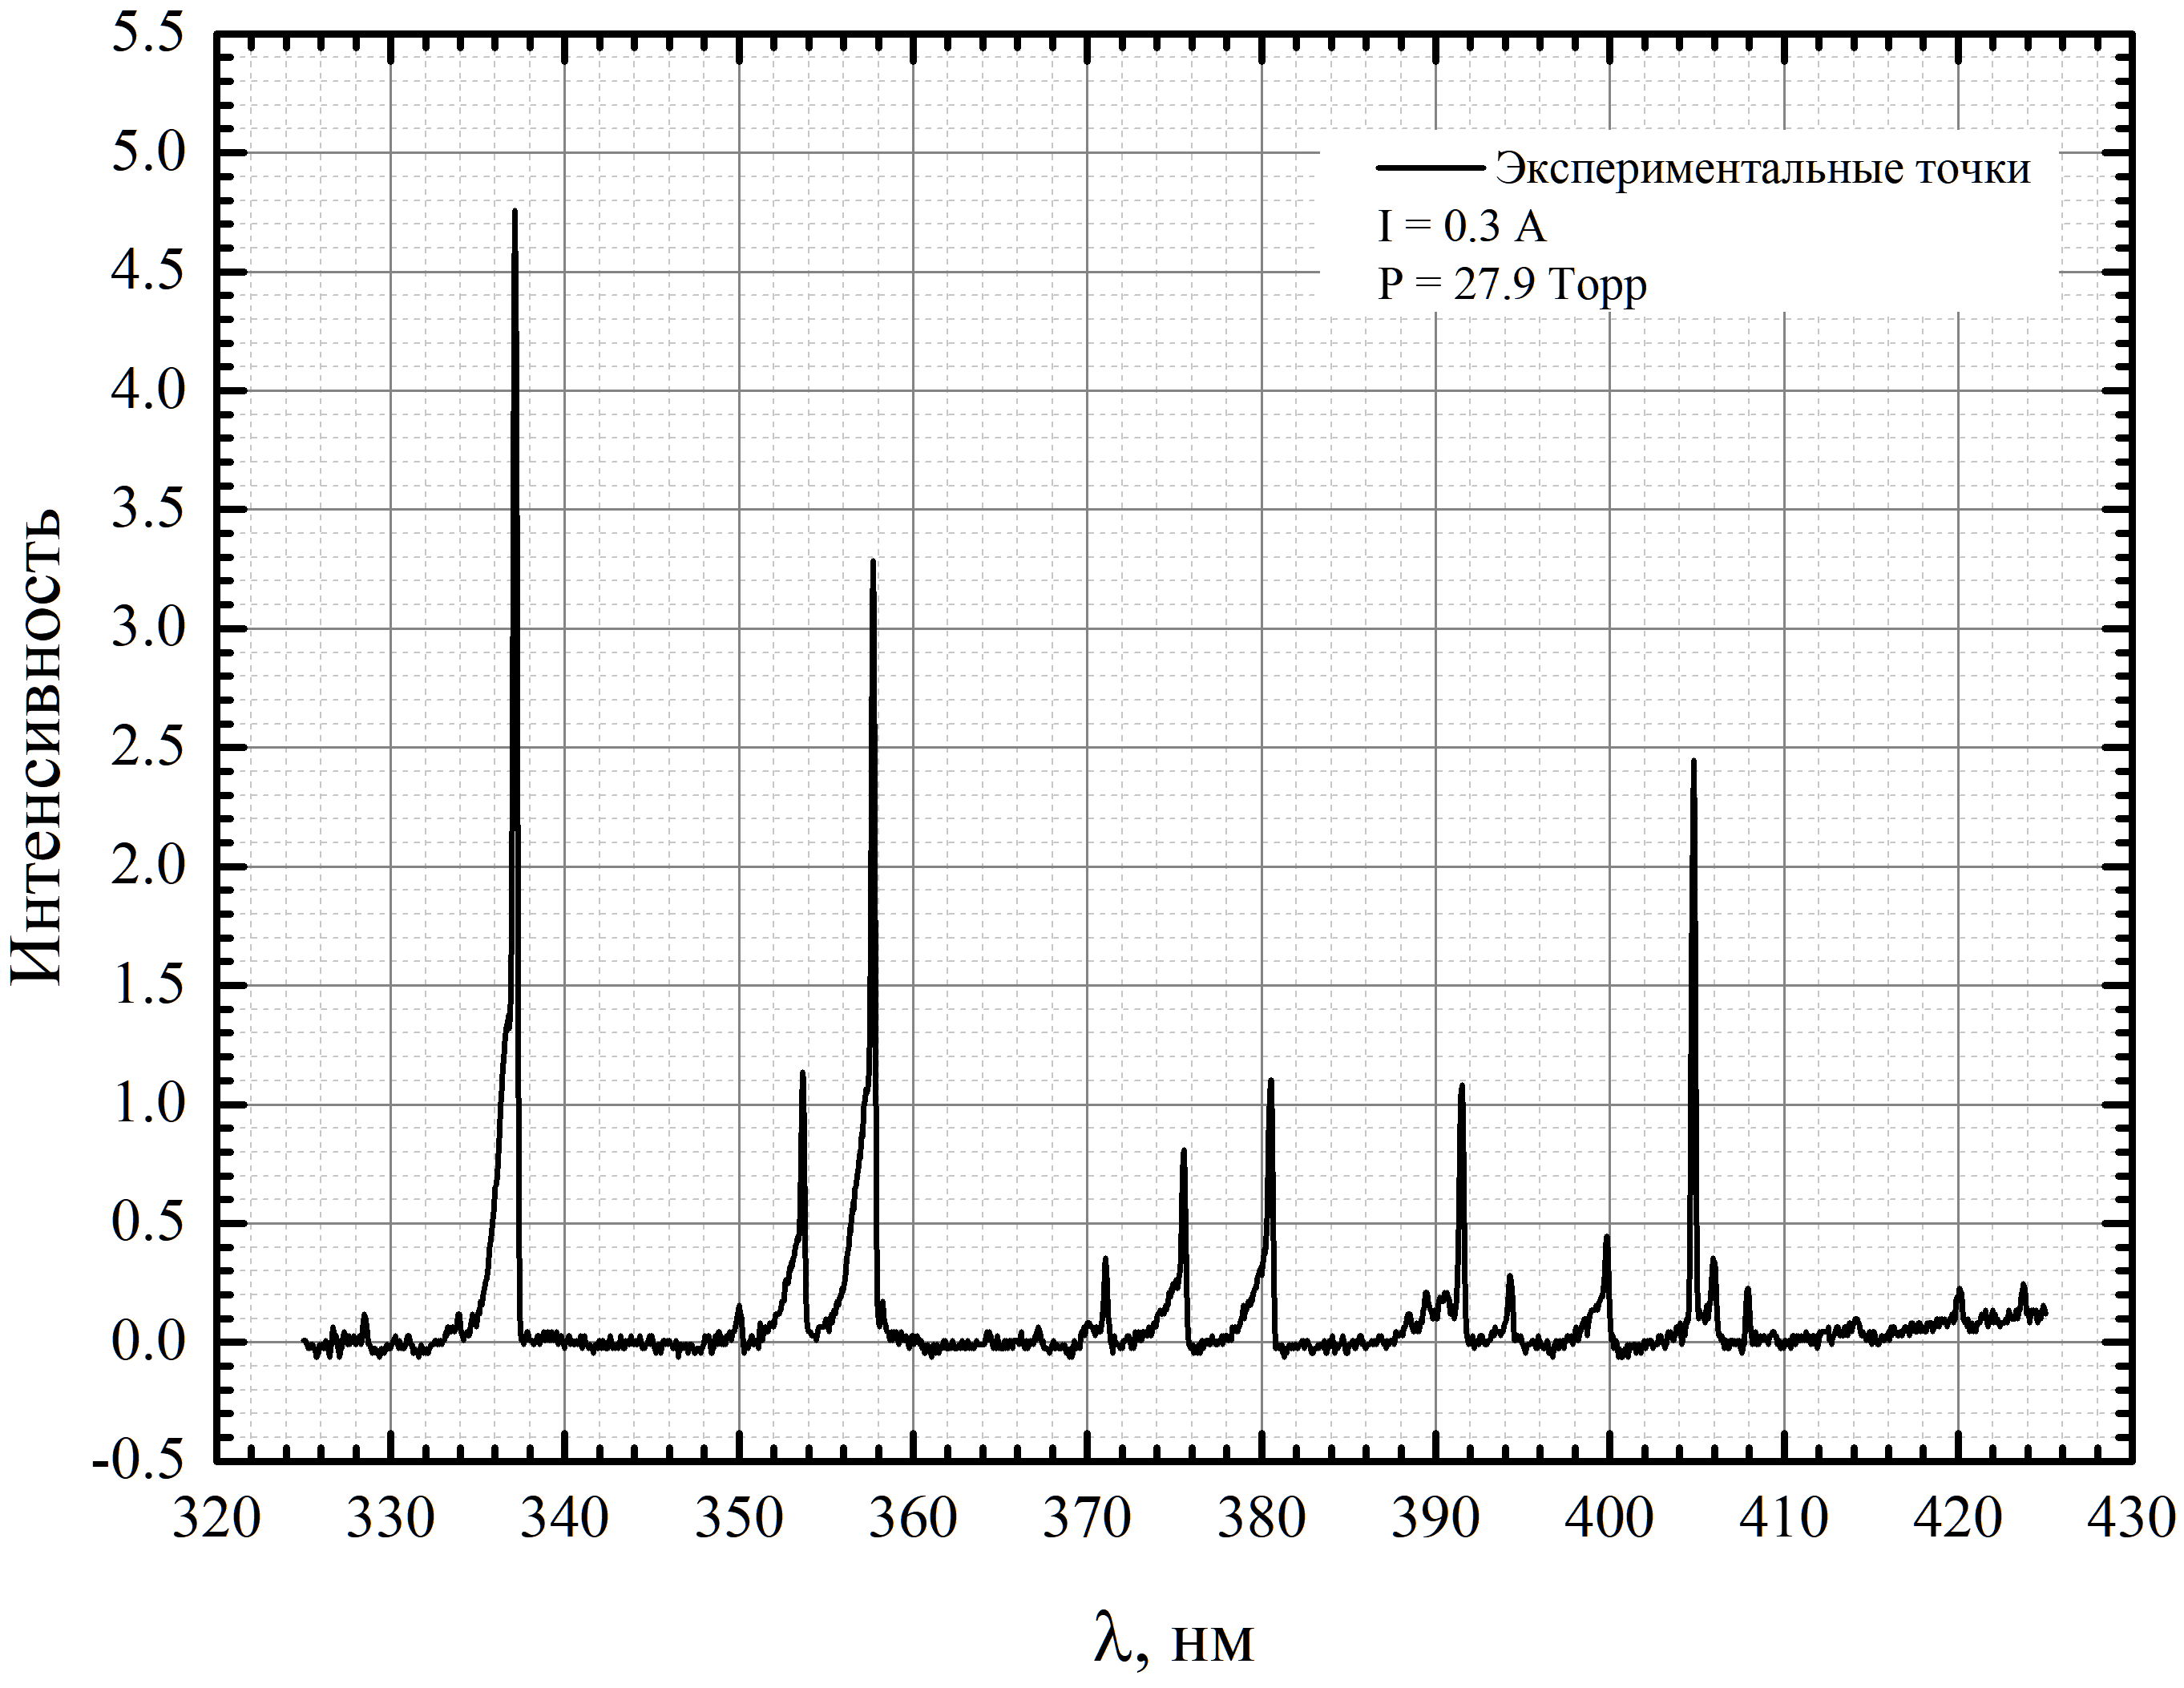
\includegraphics[width=\linewidth]{full_03_279}
		\caption{Спектр при $I= 0.3$ А, $P$= 27.9 торр}
		\label{full_03_279}
	\end{minipage} 
	\hfill
	\begin{minipage}[H]{0.45\linewidth}
		\centering
		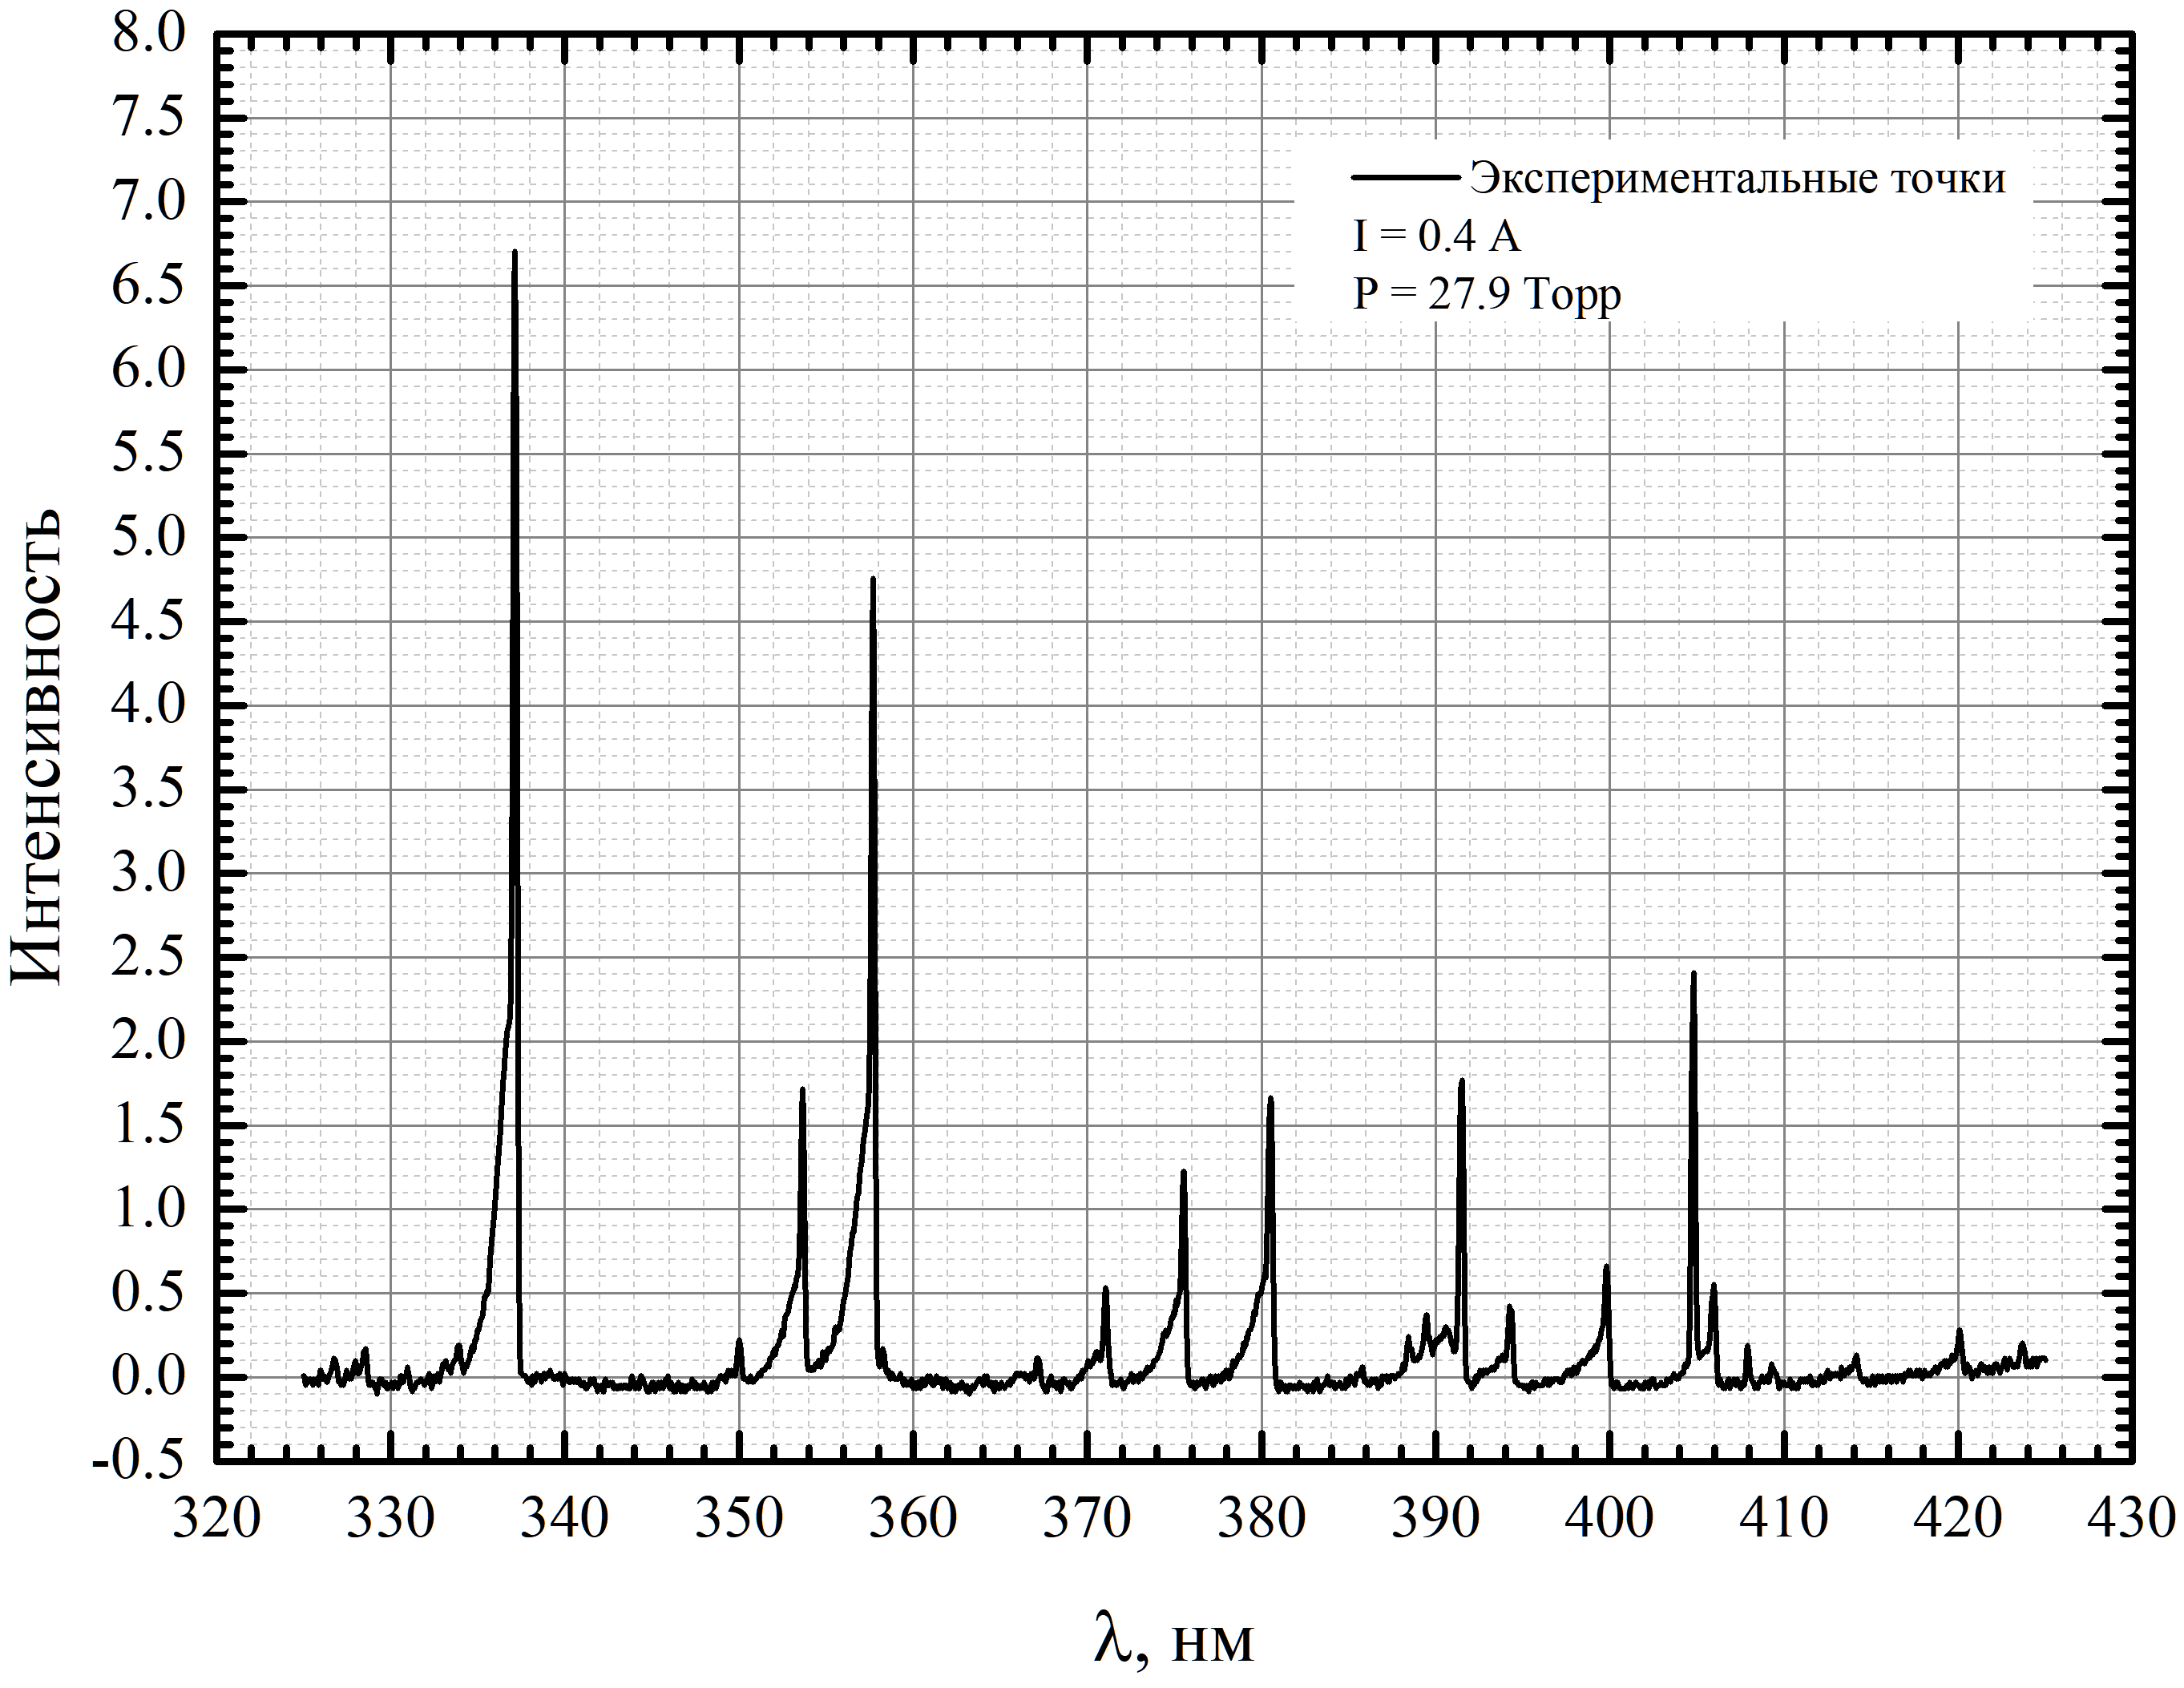
\includegraphics[width=\linewidth]{full_04_279}
		\caption{Спектр при $I= 0.4 $ А, $P$= 27.9 торр}
		\label{full_04_279}
	\end{minipage}
	\begin{minipage}{0.45\linewidth}
		\centering
		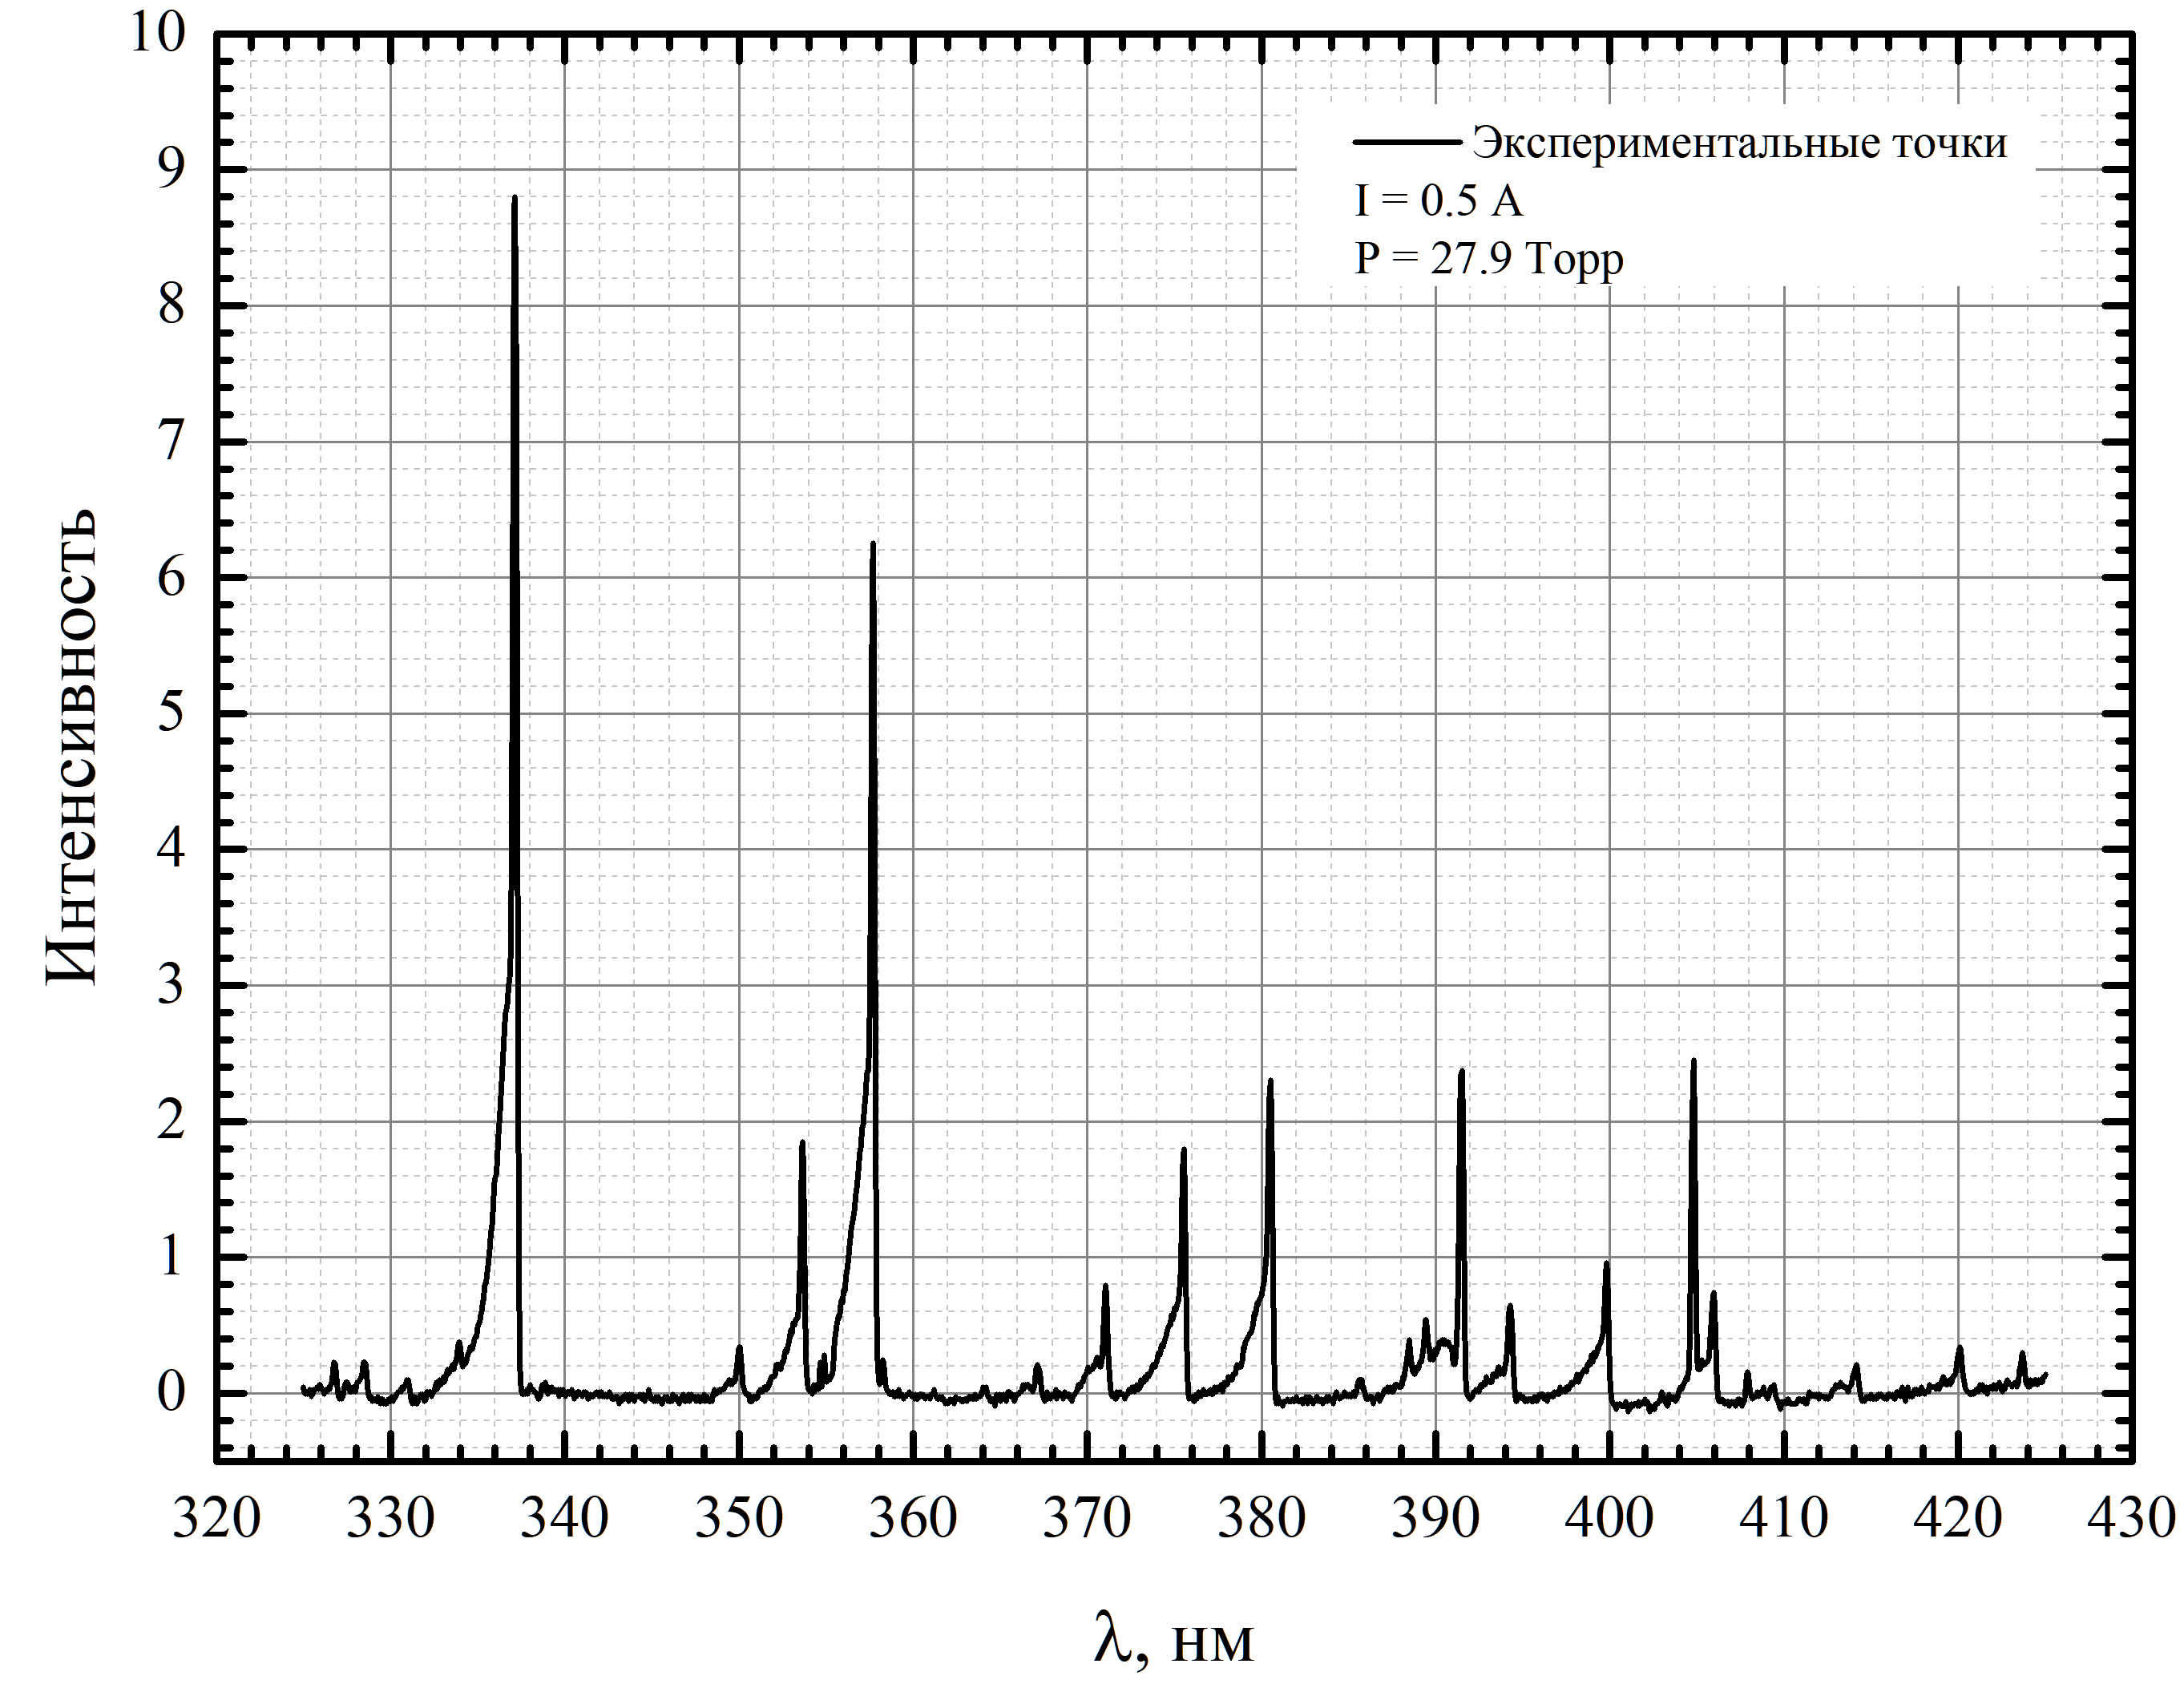
\includegraphics[width=\linewidth]{full_05_279}
		\caption{Спектр при $I= 0.5 $ А, $P$= 27.9 торр}
		\label{full_05_279}	
	\end{minipage} 
	\hfill
	\begin{minipage}[H]{0.45\linewidth}
		\centering
		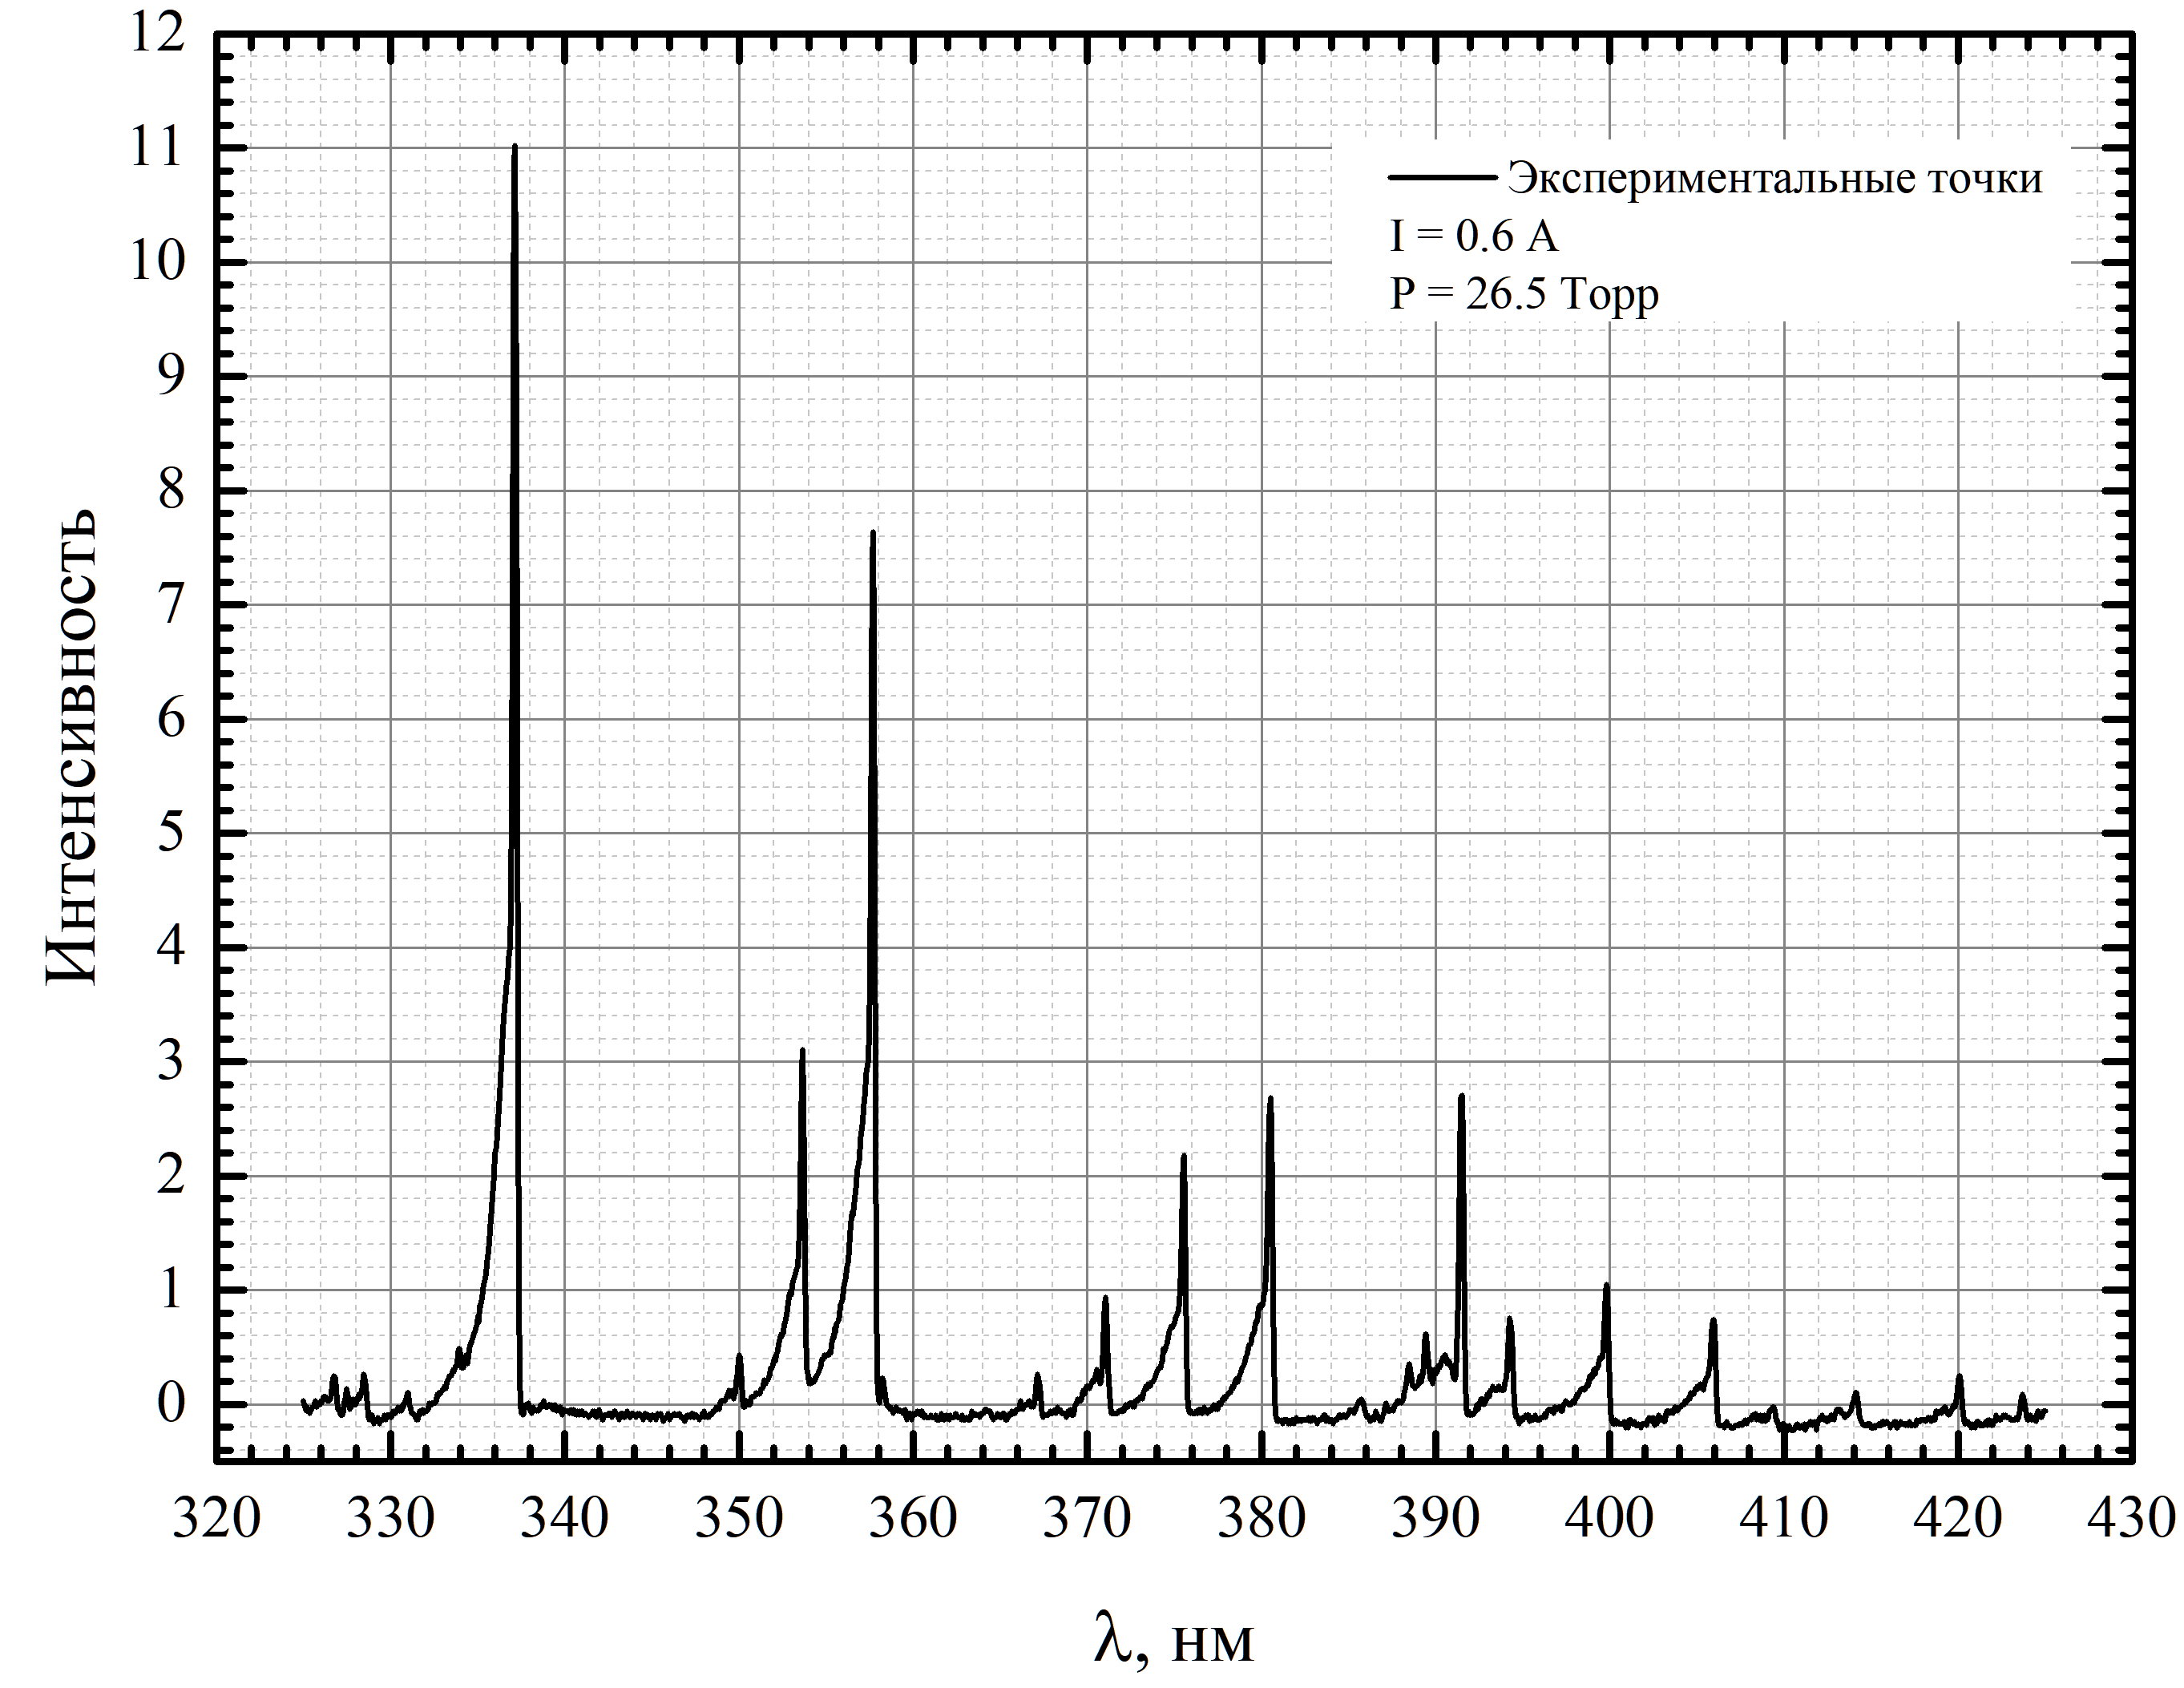
\includegraphics[width=\linewidth]{full_06_265}
		\caption{Спектр при $I= 0.6 $ А, $P$= 26.5 торр}
		\label{full_06_265}
	\end{minipage}
	\begin{minipage}{0.45\linewidth}
		\centering
		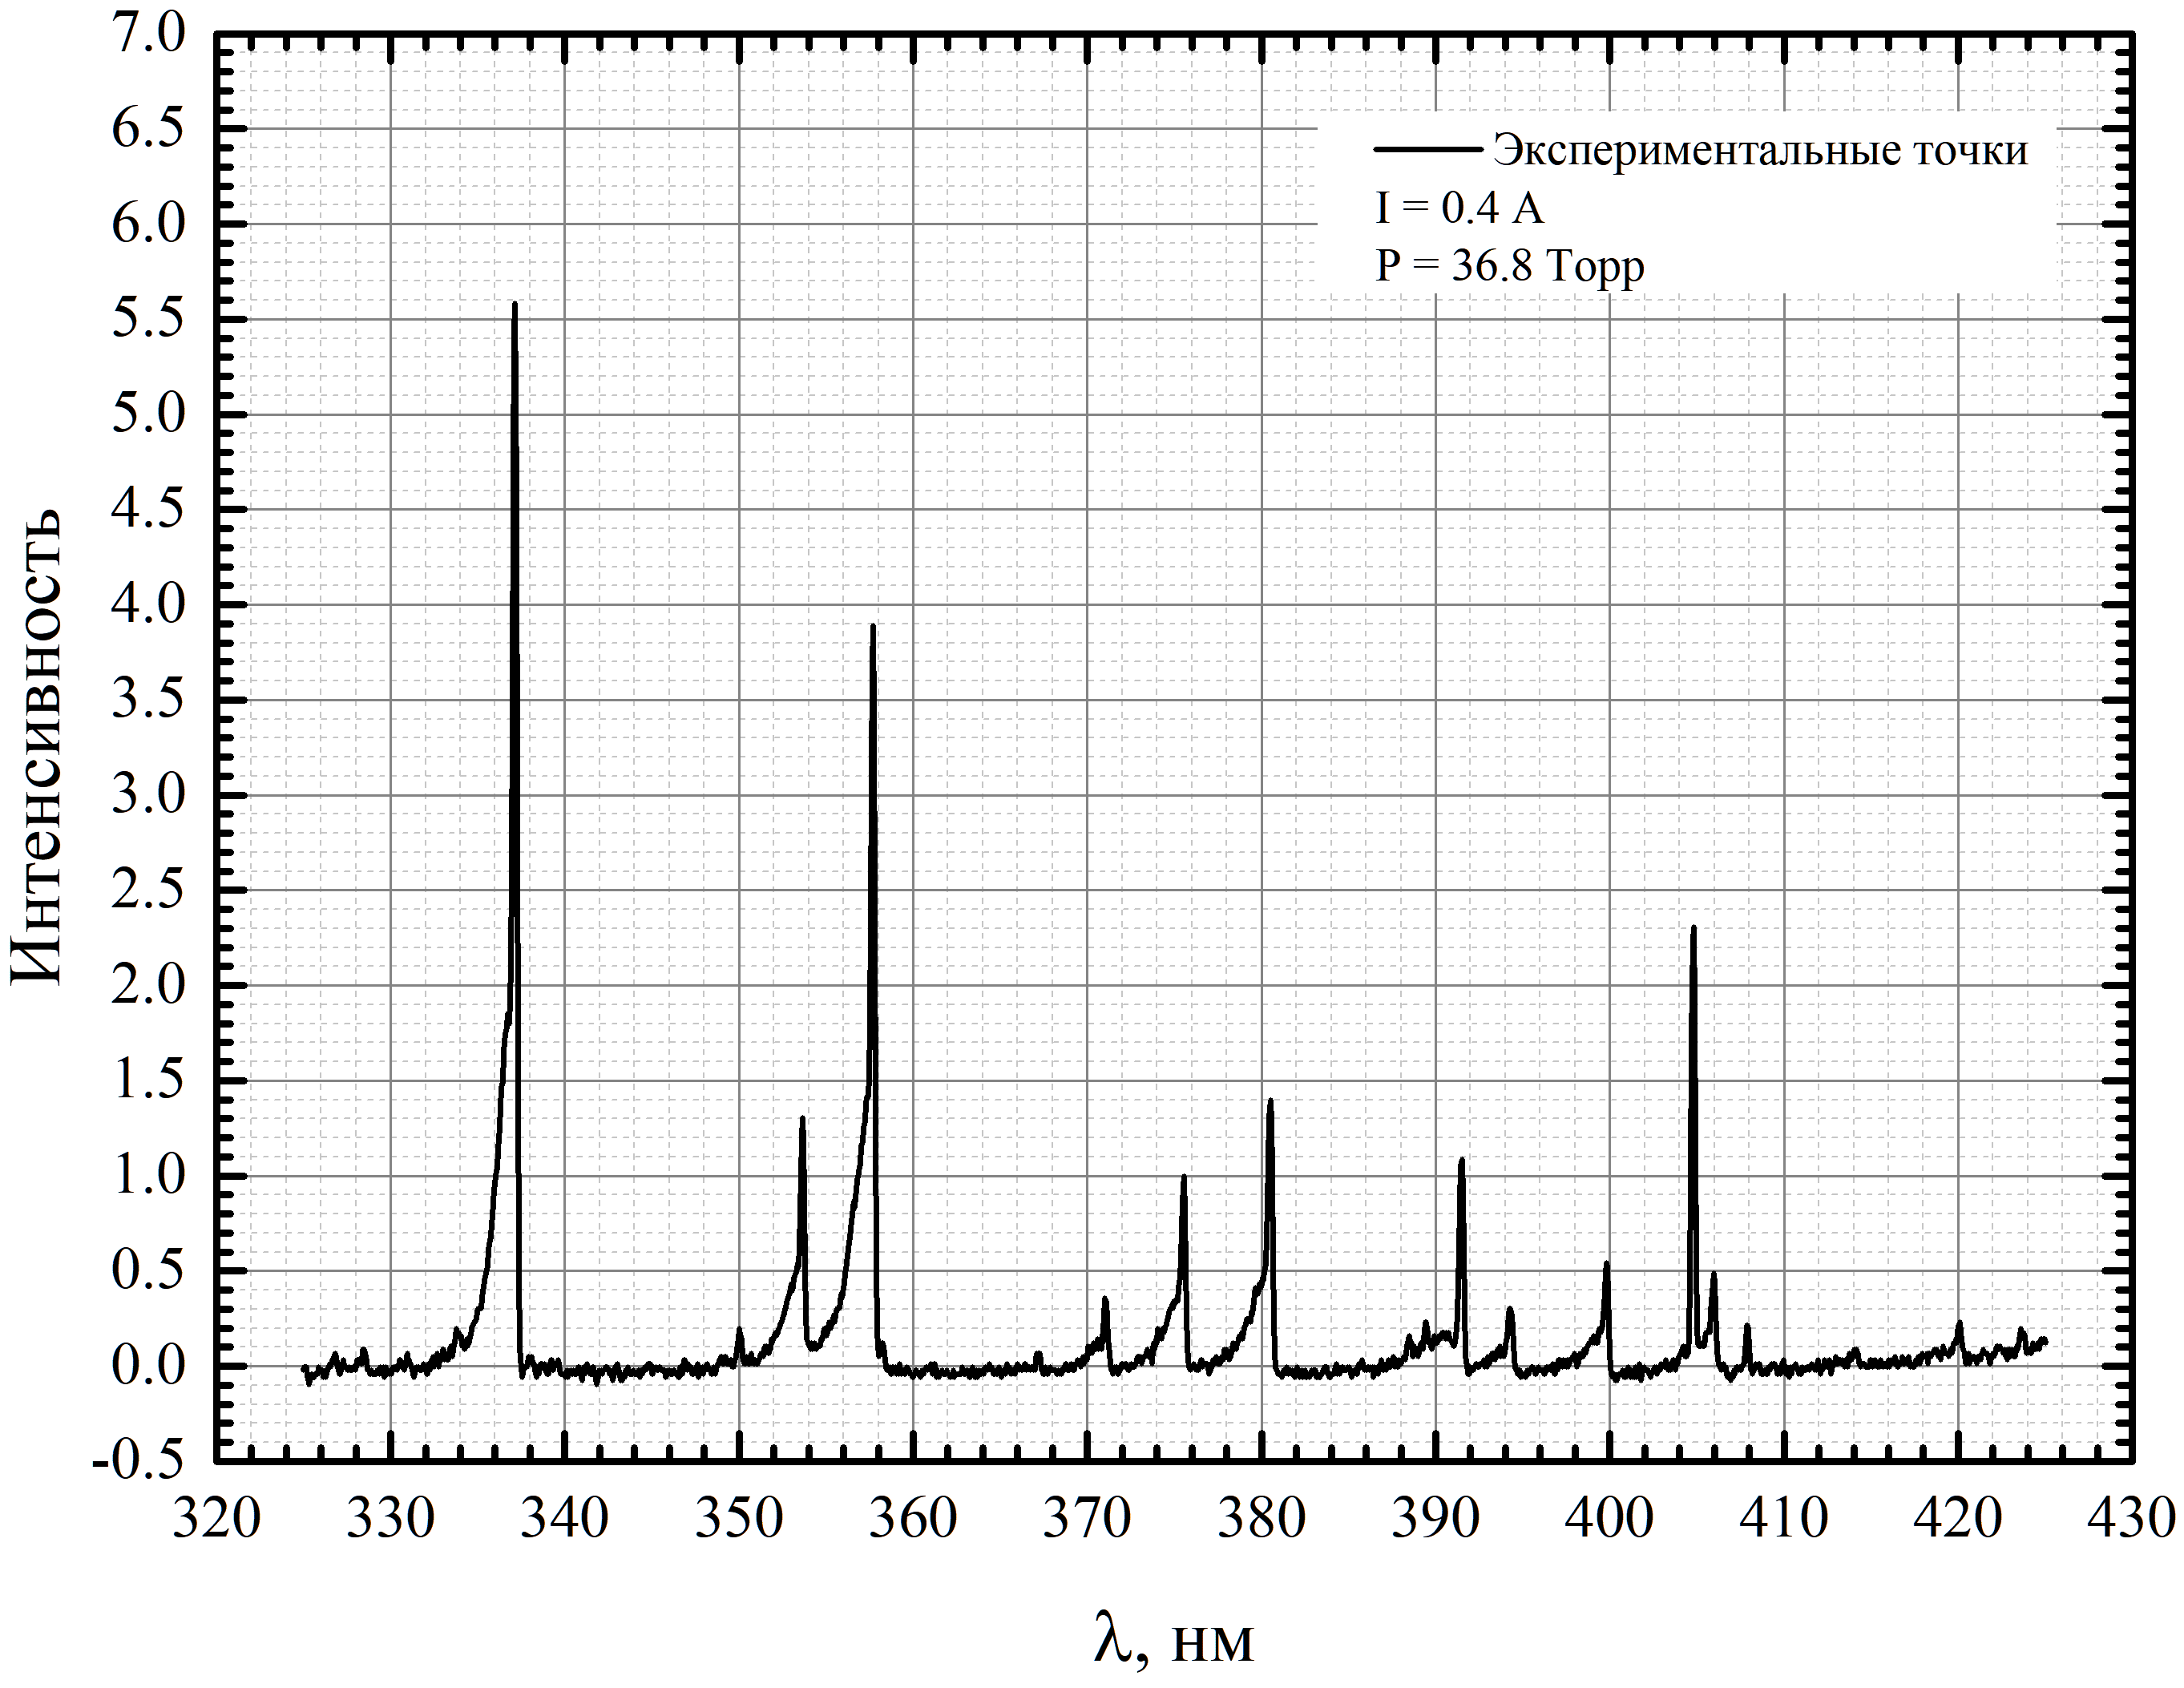
\includegraphics[width=\linewidth]{full_04_368}
		\caption{Спектр при $I= 0.4 $ А, $P$= 36.8 торр}	
		\label{full_04_368}
	\end{minipage} 
	\hfill
	\begin{minipage}[H]{0.45\linewidth}
		\centering
		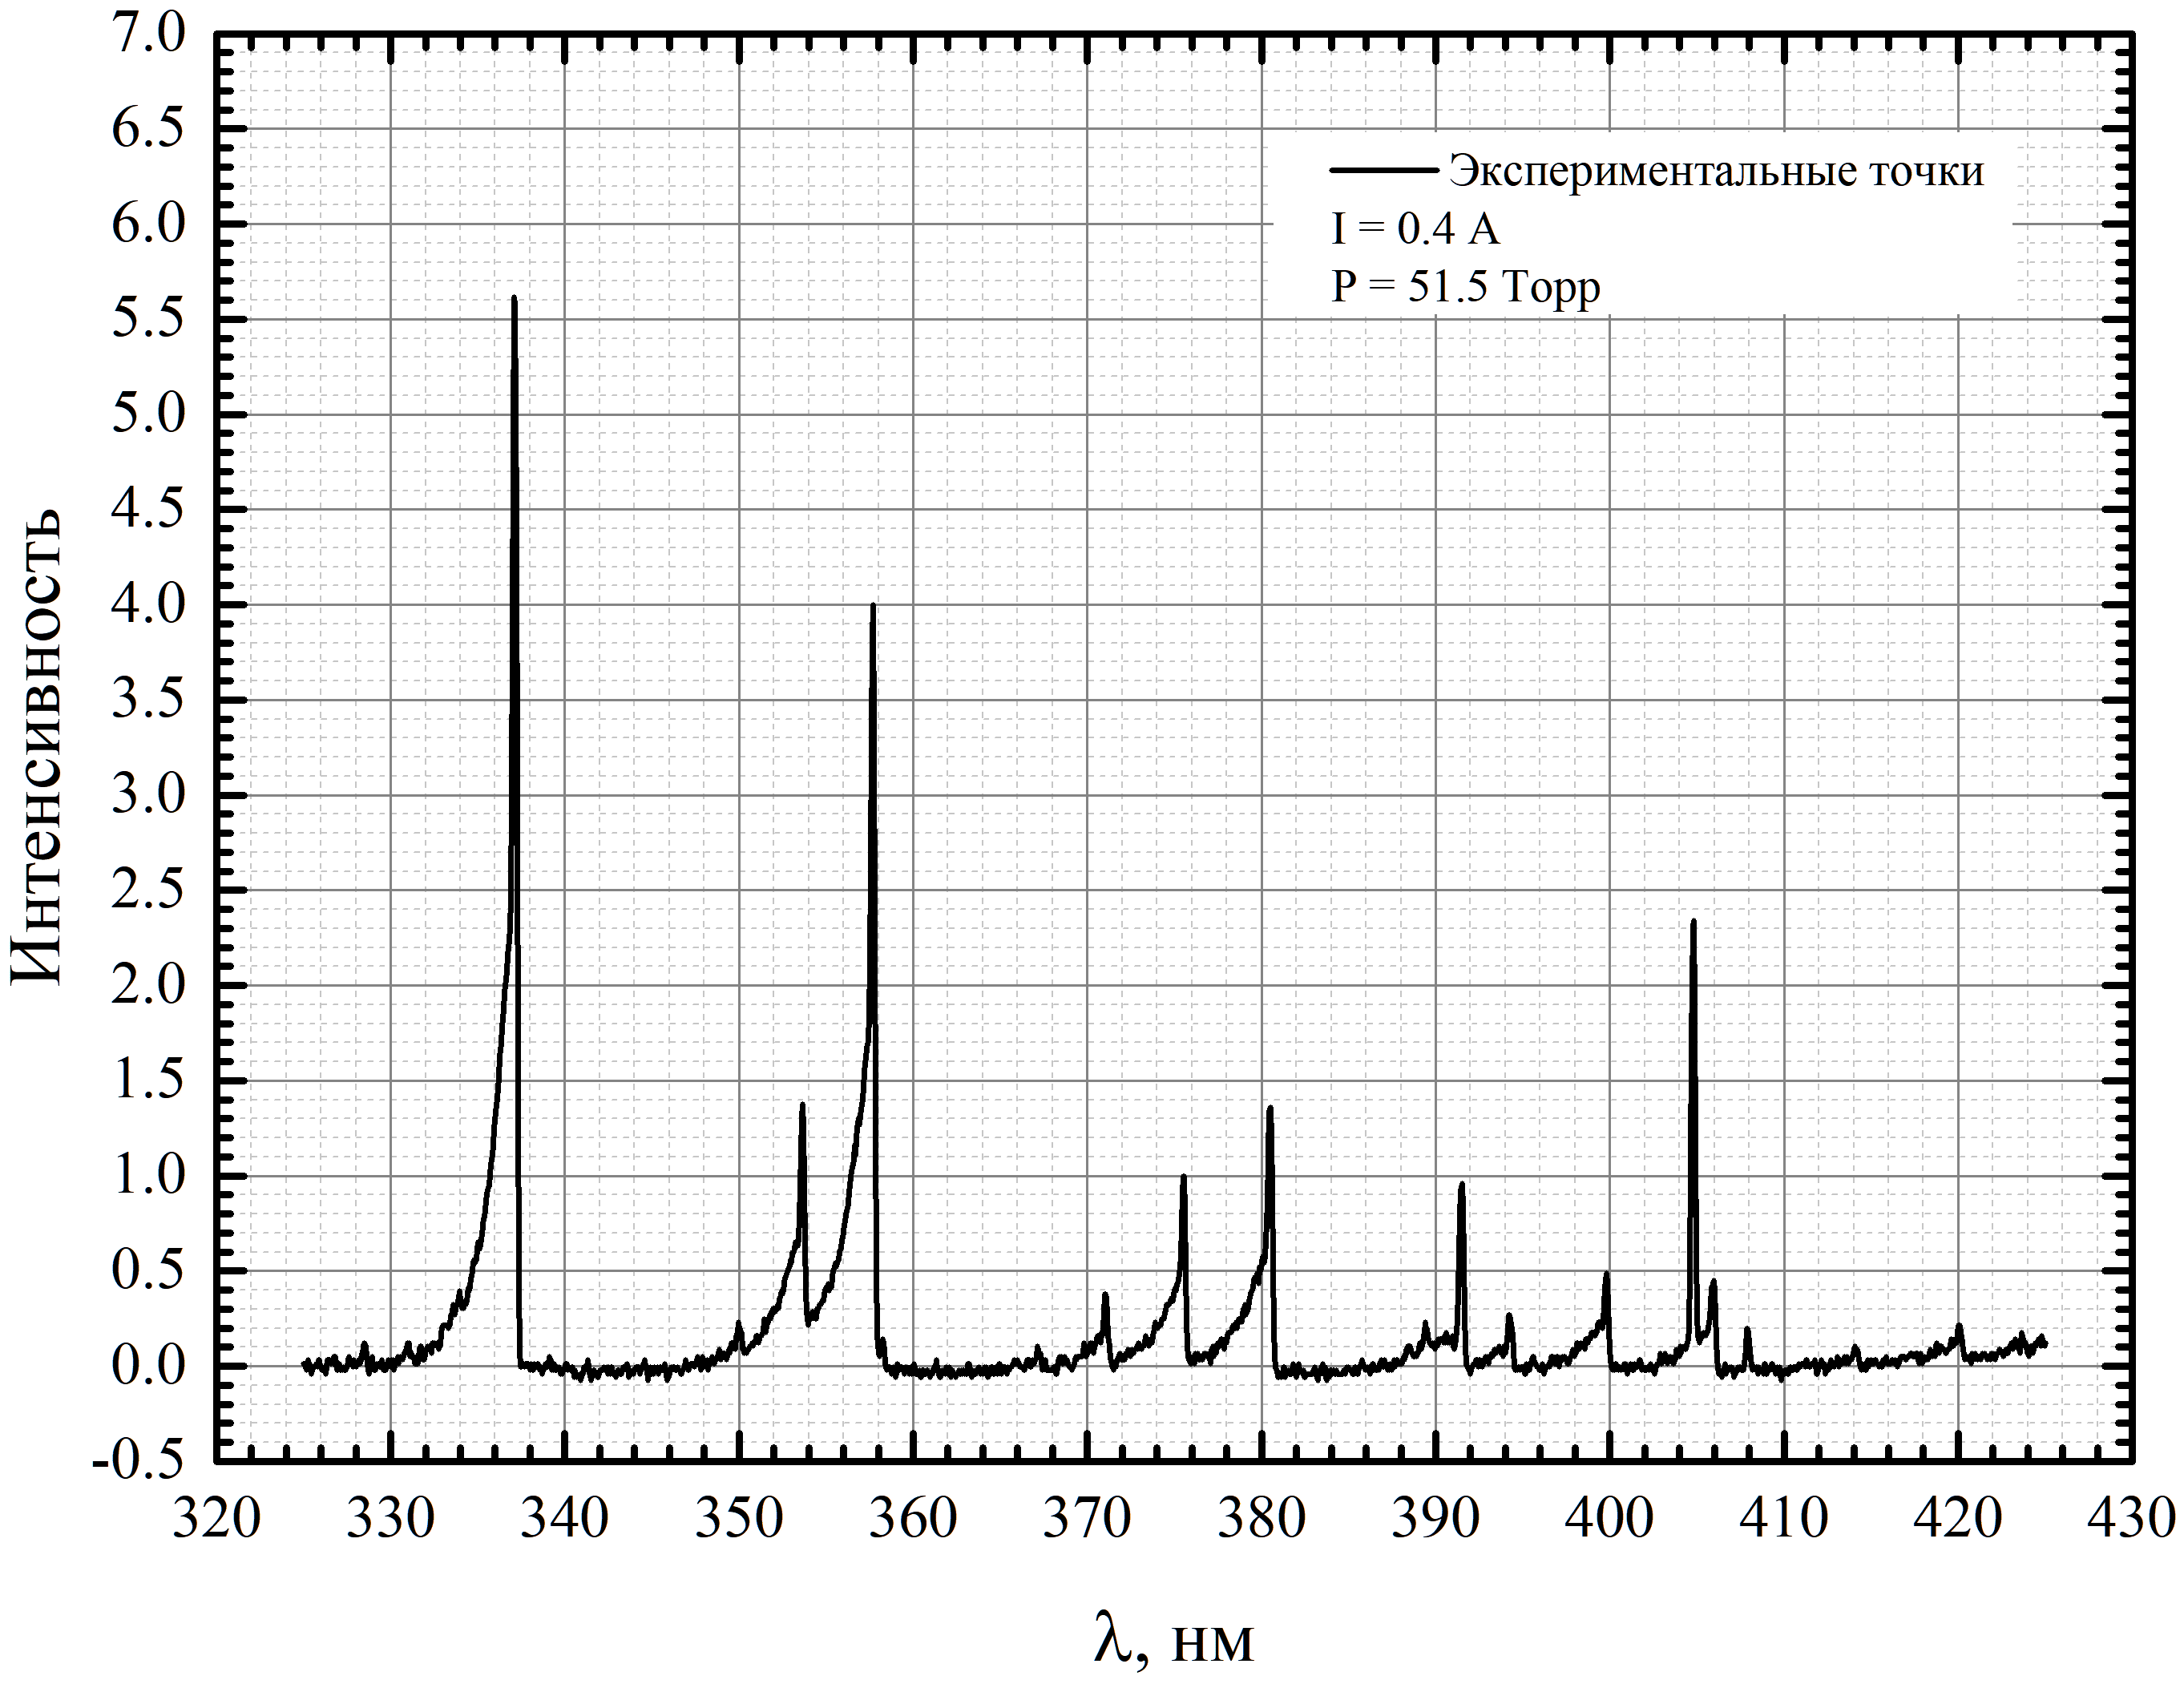
\includegraphics[width=\linewidth]{full_04_515}
		\caption{Спектр при $I= 0.6 $ А, $P$= 51.5 торр}
		\label{full_04_515}
	\end{minipage}
\end{figure}

Проведем идентификацию наблюдаемых полос (табл. \ref{tab:polosi}).

 % Table generated by Excel2LaTeX from sheet 'Лист1'
\begin{table}[H]
	\centering
	\caption{Соотнесение полос}
	\begin{tabular}{|c|c|c|c|}
		\hline
		Длина волны, \AA & Переход $v'\to v''$ & Переход $v'\to v''$ & Переход \bigstrut\\
		\hline
		4059.3 & 0$\to$3 & 3536.5 & 1$\to$2 \bigstrut\\
		\hline
		3998 & 1$\to$4 & 3500 & 2$\to$3 \bigstrut\\
		\hline
		3942.5 & 2$\to$5 & 3371.5 & 0$\to$0 \bigstrut\\
		\hline
		3805 & 0$\to$2 & 3339.5 & 1$\to$1 \bigstrut\\
		\hline
		3755.5 & 1$\to$3 & 3309.8 & 2$\to$2 \bigstrut\\
		\hline
		3710.5 & 2$\to$4 & 3284.5 & 3$\to$3 \bigstrut\\
		\hline
		3671.5 & 3$\to$5 & 3267.5 & 4$\to$4 \bigstrut\\
		\hline
		3577 & 0$\to$1 & 3258.5 & 5$\to$5 \bigstrut\\
		\hline
	\end{tabular}%
	\label{tab:polosi}%
\end{table}%

\subsection{Вычисление вращательной температуры}
Для вычисления вращательной температуры выберем участок неразрешенной
вращательной структуры и прологарифмируем его. По наклону прямой зависимости $\lg I=f(\lambda)$ , используя рассчитанную
зависимость тангенса угла наклона от значения вращательной температуры, определим значение вращательной температуры в центральной части
разряда.